\section{Versuchsauswertung}

\subsection{Solarstrahlung} 

\subsubsection{Aufnahme der Messdaten}
Zur Bestimmung der Solarstrahlung wurden folgende Halbleitersensoren und Thermosäulen in die Messdatenerfassung eingebunden:

\begin{center}
	
\begin{tabular}{ll}	
	\label{tab:Sensoren}
	Sensorname & Sensorart\\
	CM 11 & Thermosäule\\
	CM 11 (mit Schattenring) & Thermosäule\\
	CM3 & Thermosäule\\
	SSR 81 & Halbleiter\\
	TA GBS & Halbleiter
\end{tabular}
\end{center}

Der Schattenring der Thermosäule zur Messung der diffusstrahlung wurde nach Tabelle 5 des Praktikumsskriptes ausgerichtet. Die Ausrichtung der Messtafel Richtung Sonne konnte nur geschätzt werden, da der Himmel zum Zeitpunkt der Messung bedeckt war. Für die weitere Auswertung wird daher ein bereitgestellter Datensatz (vgl. Abbildung \ref{fig:radiation}) verwendet.

\begin{figure}[H]
	\centering
	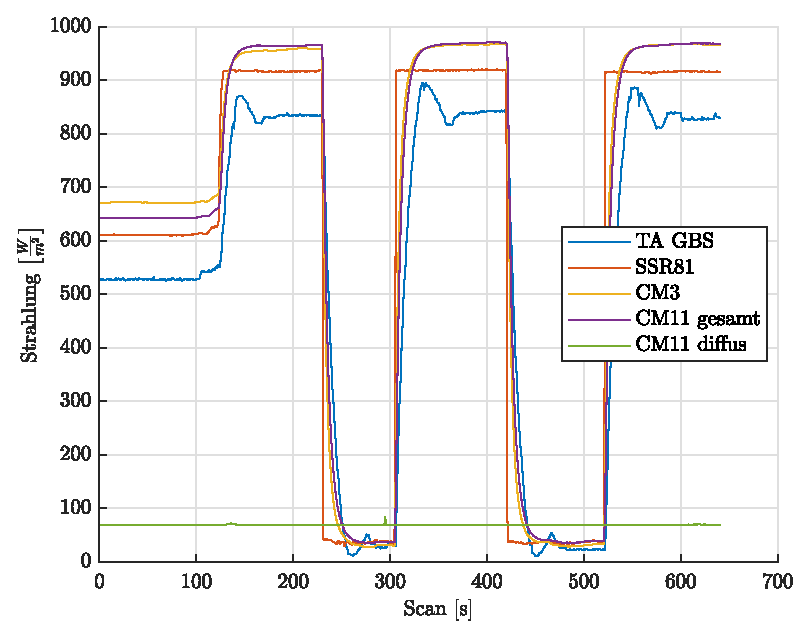
\includegraphics[width=0.8\textwidth]{../DATA/Messreihe_Strahlung.eps}
	\caption[Messreihe zur Bestimmung der Solarstrahlung]{Messreihe zur Bestimmung der Solarstrahlung}
	\label{fig:radiation}
\end{figure}
Zum Vergleich der Messwerte wurden Der Mittelwert und die Standardabweichung der einzelnen Sensoren über den stationären Messbereich zwischen Sekunde 170 und Sekunde 220 gebildet. Tabelle \ref{tab:radiation} zeigt die bestimmten Werte.
\begin{center}
\begin{tabular}{l|c|c}
	\label{tab:radiation}
	
	\textbf{Sensor} & \textbf{Strahlung [$\frac{W}{m^2}$]} & \textbf{Standardabweichung}\\
	\hline
	TA GBS & 833,6252 & 2,1081\\
	SSR81 & 916,4836 & 0,6581\\
	CM3 & 957,7781 & 1,7451\\
	CM11 & 964,5125 & 0,4149\\
	CM11 (diffus) & 68,6927 & 0,1916
\end{tabular} 
\end{center}

Die Angegeben Strahlungswerte beziehen sich auf die Globalstrahlung. Die mit einem Schattenring ausgestattete CM11 Thermosäule misst hingegen nur die Diffusstrahlung. Die Direktstrahlung kann mittels folgender Gleichung aus den beiden CM11 Thermosäulen berechnet werden:
\begin{equation}
	\label{eq:Edir}
	E_{dir}=E_{global}-E_{diffus}=\SI{964.5125}{\watt\per\square\meter}-\SI{68.692}{\watt\per\square\meter} = \SI{895.8205}{\watt\per\square\meter}
\end{equation}


\subsubsection{Bestimmung des Ansprechverhaltens}
Wie im vorherigen Teil der Auswertung wurden bereitgestellte Daten verwendet. Die Messreihe ist in Abbildung \ref{fig:response} gezeigt.
\begin{figure}[H]
	\centering
	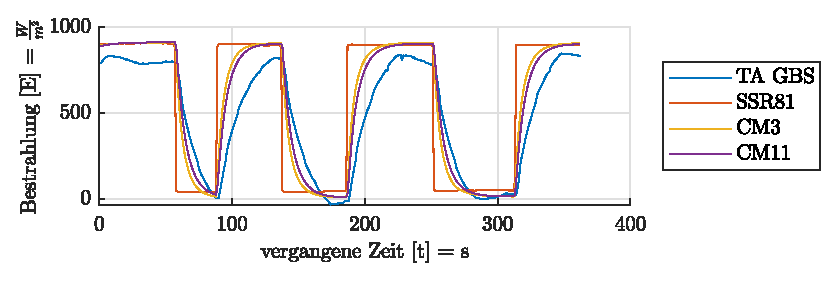
\includegraphics[width=0.8\textwidth]{../DATA/Messreihe_Ansprechzeit.eps}
	\caption[Messreihe zur Bestimmung des Ansprechverhaltens.]{Messreihe zur Bestimmung des Ansprechverhaltens.}
	\label{fig:response}
\end{figure}

\subsection{Luftfeuchtemessung}
Zunächst wurden die Umgebungstemperatur und die Ausgangsspannung des Feuchtesensors ermittelt. Abbildung \ref{fig:amb} zeigt den Messverlauf. Die Mittelwerte und Standardabweichungen sind in Tabelle \ref{tab:amb} zusammengefasst.

\begin{figure}[H]
	\centering
	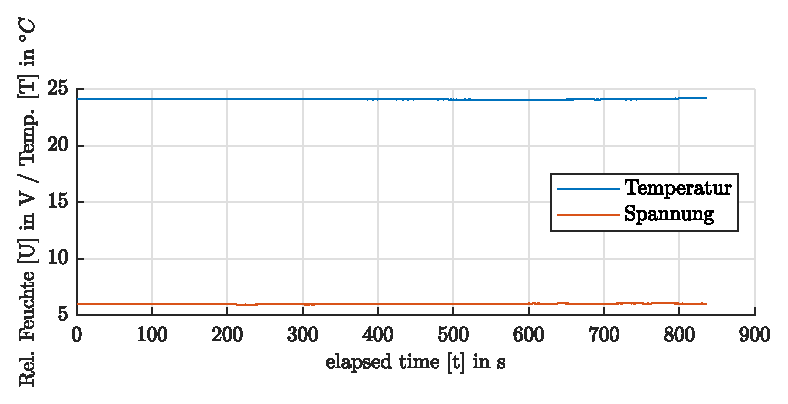
\includegraphics[width=0.8\textwidth]{../DATA/Messreihe_Umgebung.eps}
	\caption[Messreihe Umgebung]{Messreihe zur Bestimmung der Umgebungstemperatur und -luftfeuchte.}
	\label{fig:amb}
\end{figure}

\begin{center}
	\begin{tabular}{l|c|c}
		\label{tab:amb}
		
		\textbf{Messgröße} & \textbf{Mittelwerte} & \textbf{Standardabweichung}\\
		\hline
		Umgebungstemperatur & \SI{24,1005}{\celsius} & 0,0434\\
		Umgebungsluftfeuchte & 5,9791\,V & 0,0284
	\end{tabular}
\end{center}

Zur Bestimmung der relativen Feuchte wurde eine Kalibriergerade anhand zweier Messpunkte angefertigt. Hierzu wurde die Ausgangsspannung des Sensors zunächst über einer NaCl-Lösung, anschließend über einer LiCl-Lösung gemessen. Der Messverlauf ist in Abbildung \ref{fig:cal} aufgetragen. Es wurden jeweils die letzten 100 Scans zur Bestimmung der Ausgangsspannung gemittelt (vgl. Tabelle \ref{tab:cal}). Bei der vorliegenden Umgebungstemperatur von ca. \SI{24}{\celsius} entspricht die relative Luftfeuchte über NaCl 75\,\%, über LiCl 12\,\%. 

\begin{figure}[H]
	\centering
	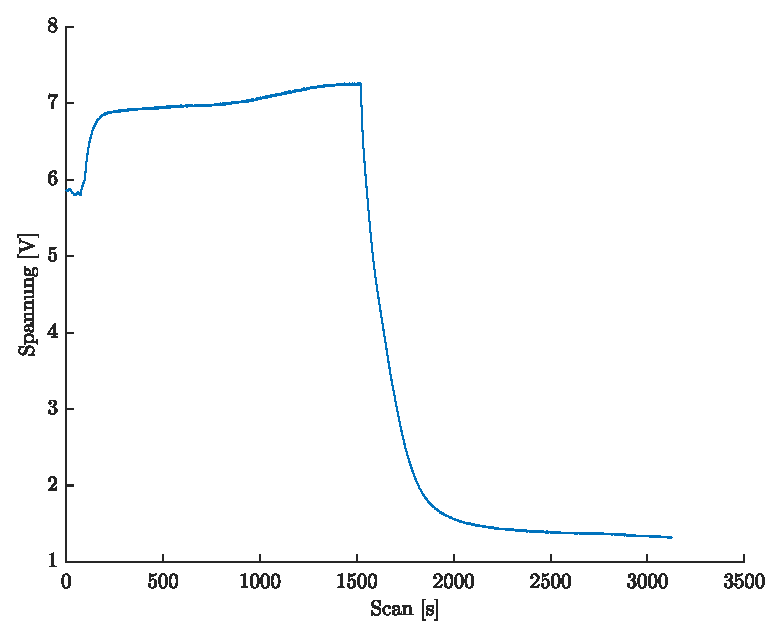
\includegraphics[width=0.8\textwidth]{../DATA/Messreihe_Feuchtekalibration.eps}
	\caption[Kalibrationsmessung]{Kalibrationsmessung anhand zweier Salzlösungen. Zum Zeitpunkt t=1500s wurde der Sensor von der NaCl-Lösung über die LiCl-Lösung überführt.}
	\label{fig:cal}
\end{figure}

\begin{center}
	\begin{tabular}{l|c|c|c}
		\label{tab:cal}
		
		\textbf{Kalibrierlösung} & \textbf{Mittelwerte} [V]& \textbf{Standardabweichung} & rel. Feuchte [\%]\\
		\hline
		LiCl & 1,3298 & 0,0052 & 12\\
		NaCl & 7,2433 & 0,0056 & 75
	\end{tabular}
\end{center}

Die Kalibriergerade (vgl. Abbildung \ref{fig:cal2}) wurde anhand der Spannungen aus Tabelle \ref{tab:cal} erstellt. Diese wird als Polynom erster Ordnung beschrieben (vgl. Gleichung \ref{eq:pol}).
\begin{equation}
	\label{eq:pol}
	\varphi(\text{V}) = p1*\text{V} + p2
\end{equation}

\begin{figure}[H]
	\centering
	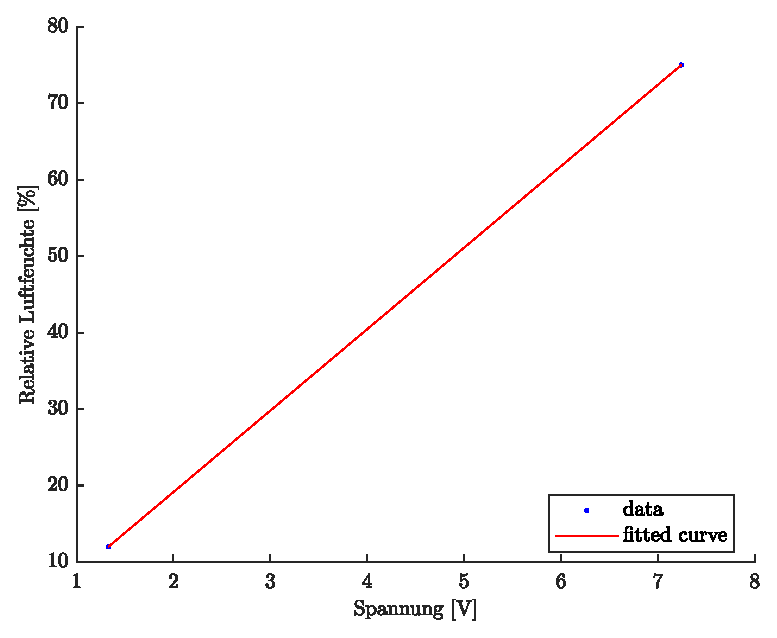
\includegraphics[width=0.8\textwidth]{../DATA/Kalibriergerade_Feuchte.eps}
	\caption[Kalibrationsgerade des Temperatursensors]{Kalibrationsgerade des Temperatursensors mit der Fit-Funktion $f(x) = p1*x + p2$ und den Parametern p1=10,65 und p2=0.2034}
	\label{fig:cal2}
\end{figure}

Die relative Feuchte der Umgebungsluft errechnet sich nach Abbildung \ref{fig:cal2} und Gleichung \ref{eq:pol} zu

\begin{equation}
	\label{eq:cal}
	\varphi(\text{V})=10,65*\SI{5,9791}{\volt}-2,167=\SI{61,51}{\percent}
\end{equation}
		

 